\section{Hadronic tau leptons}
\label{sec:ch6_tau}

\subsection{Reconstruction}

Hadronic $\tau$ decays are reconstructed from their visible decay products, consisting mainly of charged pions and photons from neutral-pion decays~\cite{ATLAS2022TauR22}.
Approximately 65\% of $\tau$ decays are hadronic, and the dominant modes contain one or three charged hadrons.
The decay products of an energetic $\tau$-lepton are collimated, producing a narrow calorimeter shower with a small number of associated tracks.
The visible object is denoted by $\tau_{\mathrm{had\text{-}vis}}$, or $\tau_{\mathrm{had}}$ in the selections below.
Its reconstructed momentum excludes the decay neutrino, which contributes to $\met$.

Tau candidates are reconstructed in the following stages~\cite{ATLAS2022TauR22}:
\begin{enumerate}
    \item \textbf{Jet seeding.} Calorimeter topological clusters are grouped with the anti-$k_t$ algorithm using a radius parameter $R=0.4$. The clusters are calibrated with local hadronic weights to correct the different responses to electromagnetic and hadronic showers~\cite{ATLAS2017TopoClusters}. These calorimeter seeds differ from the particle-flow jets used in the event selection.
    \item \textbf{Vertex association.} Tracks within $\Delta R<0.2$ of the seed direction are used to identify the production vertex. The vertex carrying the largest fraction of their scalar $\pT$ sum is selected. This association provides the reference for the candidate direction and track impact parameters.
    \item \textbf{Track classification.} Associated tracks are classified by a recurrent neural network (RNN) as tau-decay tracks, conversion tracks, other physical tracks or incorrectly reconstructed tracks. The classification reduces changes in the reconstructed charged multiplicity caused by unrelated tracks.
\end{enumerate}
Candidates with one or three tau-decay tracks are referred to as one-prong or three-prong candidates.
For three-prong decays, a secondary vertex can also be reconstructed from the decay tracks.
This displaced decay vertex is distinct from the production vertex selected in the vertex-association step.

\subsection{Identification}

Hadronic tau candidates are distinguished from quark- and gluon-initiated jets using a separate RNN discriminant~\cite{ATLAS2019TauRNN,ATLAS2022TauR22}.
Three groups of inputs are combined:
\begin{itemize}
    \item \textbf{Tracks}: their momenta, angular separations from the tau axis and displacement information.
    \item \textbf{Calorimeter clusters}: their energies, positions and shower properties.
    \item \textbf{Candidate observables}: the shower width, energy concentration, track-system mass and, for three-prong candidates, the significance of the secondary-vertex displacement.
\end{itemize}
The narrow shower and low charged multiplicity of a hadronic $\tau$ decay are thereby used together with its decay structure.
Nearby activity is included in the identification inputs, and no additional electron- or muon-style isolation working point is imposed.

The \texttt{Loose}, \texttt{Medium} and \texttt{Tight} requirements correspond to increasingly restrictive cuts on the discriminant.
Their target identification efficiencies are listed in Table~\ref{tab:ch6_tau_id}.
These efficiencies are conditional on reconstruction and do not represent the full efficiency for a generated $\tau$-lepton to pass the event selection.
The difference is visible in Figure~\ref{fig:ch6_tau_id}: at high $\pT$, the efficiency to reconstruct three separate decay tracks is reduced as their angular separations become smaller.
Baseline tau candidates are required to pass \texttt{Loose} RNN identification, and signal candidates must additionally satisfy \texttt{Tight}.

\begin{table}[htbp]
    \centering
    \caption[Target efficiencies of the hadronic tau identification working points]{Target RNN identification efficiencies for reconstructed hadronic tau candidates~\cite{ATLAS2022TauR22}.}
    \label{tab:ch6_tau_id}
    \begin{tabular}{lcc}
        \toprule
        Working point & One-prong & Three-prong \\
        \midrule
        \texttt{Loose} & 85\% & 75\% \\
        \texttt{Medium} & 75\% & 60\% \\
        \texttt{Tight} & 60\% & 45\% \\
        \bottomrule
    \end{tabular}
\end{table}

\begin{figure}[htbp]
    \centering
    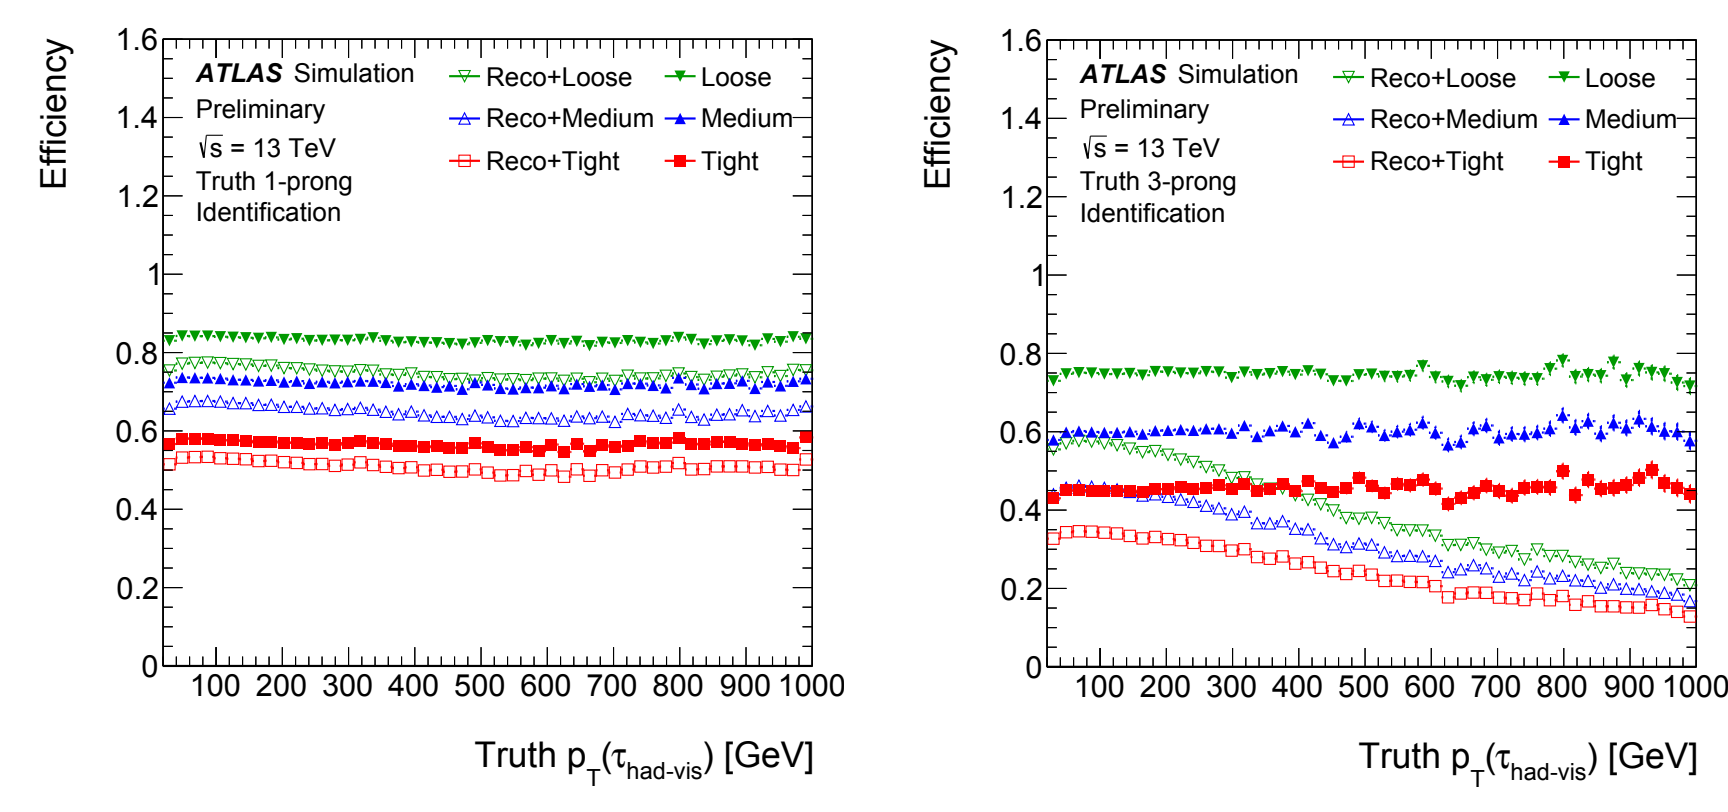
\includegraphics[width=0.82\textwidth]{output/ch6/figures/tau_identification.png}
    \caption[Hadronic tau reconstruction and identification efficiencies]{Identification efficiency alone (filled symbols) and combined reconstruction and identification efficiency (open symbols) as functions of truth visible $\pT$ for one-prong (left) and three-prong (right) hadronic tau decays in simulated $\gamma^*\rightarrow\tau\tau$ events~\cite{ATLAS2022TauR22}.}
    \label{fig:ch6_tau_id}
\end{figure}

Electrons are rejected with a separate RNN using shower and track information, including the relation between the calorimeter energy and track momentum~\cite{ATLAS2022TauR22}.
In the analysis, both baseline and signal tau candidates are required to pass the \texttt{Loose} electron-rejection working point.
Muon rejection uses the angular separation between the tau candidate and reconstructed muons.

\subsection{Calibration}

The tau energy scale is calibrated to the visible decay products using calorimeter and tracking measurements~\cite{ATLAS2022TauR22}.
The calibration is performed in three steps:
\begin{enumerate}
    \item \textbf{Calorimeter estimate.} The locally calibrated cluster energies in the tau core are corrected for pile-up and the average detector response.
    \item \textbf{Combined estimate.} A second momentum estimate is formed from charged-particle tracks and neutral calorimeter deposits. It is combined with the calorimeter estimate using weights determined by their expected resolutions.
    \item \textbf{Multivariate correction.} A boosted regression tree refines the combined estimate using shower properties, track multiplicity, reconstructed decay structure and pile-up information.
\end{enumerate}
The resulting multivariate calibration is used for the tau kinematics in this analysis.
The improvement in resolution is illustrated in Figure~\ref{fig:ch6_tau_tes}.
The decay-neutrino momentum is excluded from the calibration target.

\begin{figure}[htbp]
    \centering
    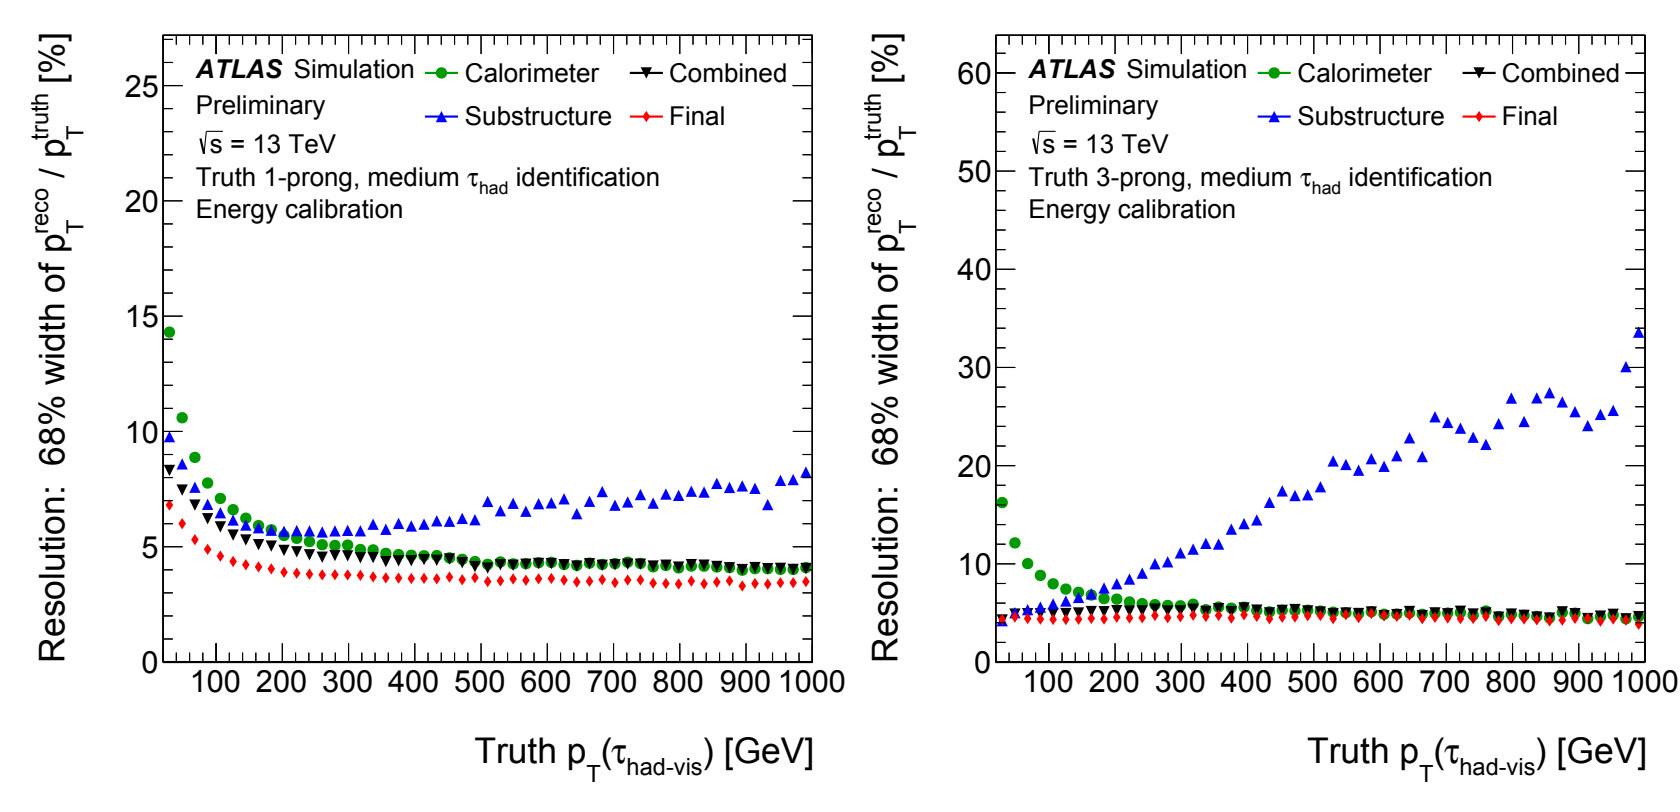
\includegraphics[width=0.82\textwidth]{output/ch6/figures/tau_energy_resolution.png}
    \caption[Hadronic tau momentum resolution and calibration]{Relative visible-momentum resolution versus truth visible $\pT$ for one-prong (left) and three-prong (right) tau candidates passing \texttt{Medium} identification in simulated $\gamma^*\rightarrow\tau\tau$ events. The resolution is half the width of the central 68\% interval of the reconstructed-to-truth $\pT$ ratio~\cite{ATLAS2022TauR22}.}
    \label{fig:ch6_tau_tes}
\end{figure}

Simulated event weights are corrected for differences in tau reconstruction, identification and electron-rejection efficiencies between data and simulation.
For signal candidates passing \texttt{Tight} tau identification, the electron-rejection scale factor associated with \texttt{Medium} tau identification is used.
